% main.tex -- ACM acmart, acmsmall (D-006). Build: pdflatex main; bibtex main; pdflatex main; pdflatex main
% Numbers and tables come from generated/ (scripts/make_paper_assets.py); never type a result by hand.
% "nonacm" drops the ACM copyright/journal block for a course paper; remove it if a venue needs the full block.
\documentclass[acmsmall,nonacm]{acmart}

\usepackage{tikz}
\usetikzlibrary{positioning}
% Generated by scripts/make_paper_assets.py from results/*.csv -- do not edit by hand.
\newcommand{\nTest}{633}
\newcommand{\nM}{118}
\newcommand{\nO}{515}
\newcommand{\nObjective}{271}
\newcommand{\auditPassed}{45}
\newcommand{\auditTotal}{45}
\newcommand{\accGreedyMain}{67.1}
\newcommand{\accGreedyMainLo}{63.5}
\newcommand{\accGreedyMainHi}{70.8}
\newcommand{\accVoteMain}{70.6}
\newcommand{\accVoteMainLo}{67.0}
\newcommand{\accVoteMainHi}{74.2}
\newcommand{\diffMain}{3.5}
\newcommand{\diffMainLo}{0.9}
\newcommand{\diffMainHi}{6.0}
\newcommand{\pMain}{0.012}
\newcommand{\bMain}{46}
\newcommand{\cMain}{24}
\newcommand{\nMainAnalysis}{633}
\newcommand{\accGreedyLenient}{68.0}
\newcommand{\accGreedyLenientLo}{64.3}
\newcommand{\accGreedyLenientHi}{71.7}
\newcommand{\accVoteLenient}{70.9}
\newcommand{\accVoteLenientLo}{67.2}
\newcommand{\accVoteLenientHi}{74.4}
\newcommand{\diffLenient}{2.9}
\newcommand{\diffLenientLo}{0.3}
\newcommand{\diffLenientHi}{5.4}
\newcommand{\pLenient}{0.036}
\newcommand{\bLenient}{42}
\newcommand{\cLenient}{24}
\newcommand{\nLenientAnalysis}{625}
\newcommand{\accGreedyObjective}{64.9}
\newcommand{\accGreedyObjectiveLo}{59.4}
\newcommand{\accGreedyObjectiveHi}{70.5}
\newcommand{\accVoteObjective}{71.2}
\newcommand{\accVoteObjectiveLo}{65.7}
\newcommand{\accVoteObjectiveHi}{76.8}
\newcommand{\diffObjective}{6.3}
\newcommand{\diffObjectiveLo}{2.2}
\newcommand{\diffObjectiveHi}{10.7}
\newcommand{\pObjective}{0.006}
\newcommand{\bObjective}{26}
\newcommand{\cObjective}{9}
\newcommand{\nObjectiveAnalysis}{271}
\newcommand{\accGreedyM}{66.9}
\newcommand{\accGreedyMLo}{58.5}
\newcommand{\accGreedyMHi}{75.4}
\newcommand{\accVoteM}{72.0}
\newcommand{\accVoteMLo}{63.6}
\newcommand{\accVoteMHi}{79.7}
\newcommand{\diffM}{5.1}
\newcommand{\diffMLo}{$-$1.7}
\newcommand{\diffMHi}{11.9}
\newcommand{\pM}{0.21}
\newcommand{\bM}{11}
\newcommand{\cM}{5}
\newcommand{\nMAnalysis}{118}
\newcommand{\accGreedyO}{67.2}
\newcommand{\accGreedyOLo}{63.1}
\newcommand{\accGreedyOHi}{71.3}
\newcommand{\accVoteO}{70.3}
\newcommand{\accVoteOLo}{66.4}
\newcommand{\accVoteOHi}{74.2}
\newcommand{\diffO}{3.1}
\newcommand{\diffOLo}{0.4}
\newcommand{\diffOHi}{5.8}
\newcommand{\pO}{0.040}
\newcommand{\bO}{35}
\newcommand{\cO}{19}
\newcommand{\nOAnalysis}{515}
\newcommand{\accSingle}{68.1}
\newcommand{\accSingleSD}{0.55}
\newcommand{\accSingleMin}{67.0}
\newcommand{\accSingleMax}{68.7}
\newcommand{\accKOne}{68.4}
\newcommand{\accKThree}{70.1}
\newcommand{\accKFive}{71.4}
\newcommand{\accKSeven}{70.3}
\newcommand{\accKNine}{70.3}
\newcommand{\accKTen}{70.6}
\newcommand{\unanimity}{49.4}
\newcommand{\unanimityLo}{45.5}
\newcommand{\unanimityHi}{53.2}
\newcommand{\modalShare}{0.858}
\newcommand{\modalShareLo}{0.843}
\newcommand{\modalShareHi}{0.872}
\newcommand{\kappaRuns}{0.715}
\newcommand{\kappaRunsLo}{0.689}
\newcommand{\kappaRunsHi}{0.738}
\newcommand{\flipRate}{21.4}
\newcommand{\flipRateLo}{19.5}
\newcommand{\flipRateHi}{23.3}
\newcommand{\auroc}{0.737}
\newcommand{\aurocLo}{0.695}
\newcommand{\aurocHi}{0.780}
\newcommand{\accGeNine}{83.5}
\newcommand{\nGeNine}{406}
\newcommand{\accLtNine}{47.6}
\newcommand{\nLtNine}{227}
\newcommand{\coverageTen}{49.4}
\newcommand{\accTen}{86.9}
\newcommand{\unpGreedyPct}{1.3}
\newcommand{\unpSampledPct}{0.6}
\newcommand{\truncGreedyPct}{1.1}
\newcommand{\truncSampledPct}{0.6}
\newcommand{\ties}{25}
\newcommand{\unpGreedyN}{8}
\newcommand{\unpGreedyTruncN}{7}
\newcommand{\runsGreedyN}{633}
\newcommand{\unpSampledN}{40}
\newcommand{\unpSampledTruncN}{36}
\newcommand{\runsSampledN}{6{,}330}
\newcommand{\tokGreedyItem}{248}
\newcommand{\tokVoteItem}{2{,}491}
\newcommand{\tokRatio}{10.0}
\newcommand{\gpuGreedy}{428}
\newcommand{\gpuVote}{1{,}580}
\newcommand{\gpuRatio}{3.7}
\newcommand{\rerunFiftySame}{48}
\newcommand{\rerunSamePct}{98.7}
\newcommand{\rerunSame}{625}
\newcommand{\rerunDiff}{$-$0.6}
\newcommand{\rerunDiffLo}{$-$1.6}
\newcommand{\rerunDiffHi}{0.2}
\newcommand{\rerunP}{0.29}
\newcommand{\accRerun}{66.5}
\newcommand{\diffTLow}{2.4}
\newcommand{\diffTLowLo}{0.2}
\newcommand{\diffTLowHi}{4.6}
\newcommand{\pTLow}{0.063}
\newcommand{\accVoteTLow}{69.5}
\newcommand{\unanimityTLow}{54.0}
\newcommand{\aurocTLow}{0.721}
\newcommand{\diffTHigh}{3.8}
\newcommand{\diffTHighLo}{0.9}
\newcommand{\diffTHighHi}{6.6}
\newcommand{\pTHigh}{0.013}
\newcommand{\accVoteTHigh}{70.9}
\newcommand{\unanimityTHigh}{47.6}
\newcommand{\aurocTHigh}{0.748}
\newcommand{\probeHits}{4}
\newcommand{\probeN}{100}
\newcommand{\probeLo}{1.6}
\newcommand{\probeHi}{9.8}
\newcommand{\bGreedyLetterRuns}{2.5}
\newcommand{\bKeyRuns}{6.8}
\newcommand{\cKeyRuns}{3.0}
\newcommand{\tiesB}{5}
\newcommand{\tiesC}{6}
\newcommand{\bGreedyUnparseable}{4}
\newcommand{\allWrong}{78}
\newcommand{\allWrongSame}{41}
\newcommand{\allWrongMixed}{35}
\newcommand{\allWrongUnparseable}{2}
\newcommand{\unanimousWrong}{41}
\newcommand{\unanimousN}{313}
\newcommand{\unanimousWrongPct}{13.1}
\newcommand{\stableTLow}{67.0}
\newcommand{\stableTMid}{64.1}
\newcommand{\stableTHigh}{62.2}
\newcommand{\voteVsRerun}{4.1}
\newcommand{\voteVsRerunLo}{1.6}
\newcommand{\voteVsRerunHi}{6.6}
\newcommand{\voteVsRerunP}{0.003}
\newcommand{\decompSingle}{0.9}
\newcommand{\decompSingleLo}{$-$1.2}
\newcommand{\decompSingleHi}{3.1}
\newcommand{\decompVote}{2.6}
\newcommand{\decompVoteLo}{1.1}
\newcommand{\decompVoteHi}{4.0}
\newcommand{\voteEachMin}{1.9}
\newcommand{\voteEachMax}{3.6}
\newcommand{\voteEachB}{39--49}
\newcommand{\voteEachC}{21--35}
\newcommand{\voteEachP}{0.007--0.17}
\newcommand{\discordancePct}{11.1}
\newcommand{\nOriginTrain}{492}
\newcommand{\accGreedyOriginTrain}{66.3}
\newcommand{\accVoteOriginTrain}{69.7}
\newcommand{\diffOriginTrain}{3.5}
\newcommand{\diffOriginTrainLo}{0.4}
\newcommand{\diffOriginTrainHi}{6.5}
\newcommand{\bOriginTrain}{37}
\newcommand{\cOriginTrain}{20}
\newcommand{\pOriginTrain}{0.033}
\newcommand{\nOriginDev}{70}
\newcommand{\accGreedyOriginDev}{65.7}
\newcommand{\accVoteOriginDev}{68.6}
\newcommand{\diffOriginDev}{2.9}
\newcommand{\diffOriginDevLo}{$-$4.3}
\newcommand{\diffOriginDevHi}{11.4}
\newcommand{\bOriginDev}{5}
\newcommand{\cOriginDev}{3}
\newcommand{\pOriginDev}{0.73}
\newcommand{\nOriginTest}{71}
\newcommand{\accGreedyOriginTest}{74.6}
\newcommand{\accVoteOriginTest}{78.9}
\newcommand{\diffOriginTest}{4.2}
\newcommand{\diffOriginTestLo}{$-$1.4}
\newcommand{\diffOriginTestHi}{11.3}
\newcommand{\bOriginTest}{4}
\newcommand{\cOriginTest}{1}
\newcommand{\pOriginTest}{0.38}
\newcommand{\unanDiffLowMid}{4.6}
\newcommand{\unanDiffLowMidLo}{1.4}
\newcommand{\unanDiffLowMidHi}{7.7}
\newcommand{\unanDiffHighMid}{$-$1.9}
\newcommand{\unanDiffHighMidLo}{$-$5.2}
\newcommand{\unanDiffHighMidHi}{1.4}
\newcommand{\unanDiffHighLow}{$-$6.5}
\newcommand{\unanDiffHighLowLo}{$-$9.6}
\newcommand{\unanDiffHighLowHi}{$-$3.5}
\newcommand{\aurocFirstThree}{0.644}
\newcommand{\aurocFirstThreeLo}{0.604}
\newcommand{\aurocFirstThreeHi}{0.685}
\newcommand{\aurocGreedyAgree}{0.586}
\newcommand{\aurocGreedyAgreeLo}{0.551}
\newcommand{\aurocGreedyAgreeHi}{0.621}
\newcommand{\aurocGreedyCorrect}{0.749}
\newcommand{\aurocGreedyCorrectLo}{0.709}
\newcommand{\aurocGreedyCorrectHi}{0.788}
\newcommand{\wrongAGreedy}{34}
\newcommand{\wrongAGreedyExp}{45.3}
\newcommand{\wrongGreedyN}{200}
\newcommand{\wrongASampled}{315}
\newcommand{\wrongASampledExp}{463.3}
\newcommand{\wrongSampledN}{1{,}982}
\newcommand{\wrongLettersP}{0.10}
\newcommand{\accGreedyKeyA}{56.3}
\newcommand{\accGreedyKeyOtherMin}{68.1}
\newcommand{\accGreedyKeyOtherMax}{73.2}
\newcommand{\accVoteKeyA}{60.9}
\newcommand{\accVoteKeyOtherMin}{71.9}
\newcommand{\accVoteKeyOtherMax}{75.0}
\newcommand{\accKOrdOne}{68.0}
\newcommand{\accKOrdThree}{69.8}
\newcommand{\accKOrdFive}{70.5}
\newcommand{\accKOrdTen}{70.9}
\newcommand{\probeShortHits}{3}
\newcommand{\probeShortN}{54}
\newcommand{\probeLongHits}{1}
\newcommand{\probeLongN}{46}
\newcommand{\bGreedyLetterRunsParsed}{2.7}
\newcommand{\bParsedN}{42}
\newcommand{\pairAgree}{78.6}
\newcommand{\unpGreedyNotTruncN}{1}
\newcommand{\unpSampledNotTruncN}{4}
\newcommand{\medqaN}{12{,}723}
\newcommand{\poolN}{1{,}026}
\newcommand{\codeM}{129}
\newcommand{\codeO}{583}
\newcommand{\codeX}{314}
\newcommand{\eligibleN}{712}
\newcommand{\excludedN}{54}
\newcommand{\finalN}{658}
\newcommand{\debugN}{25}
\newcommand{\debugM}{5}
\newcommand{\screenN}{205}
\newcommand{\screenAgree}{190}
\newcommand{\screenKappa}{0.873}
\newcommand{\adjudicatedN}{15}
\newcommand{\adjudicatedChanged}{8}
\newcommand{\screenChangedPct}{3.9}
\newcommand{\unsampledN}{821}
\newcommand{\genHoursMain}{0.57}
\newcommand{\sessionHoursMain}{0.76}
\newcommand{\genHoursExtras}{0.95}
\newcommand{\sessionHoursExtras}{1.11}
\newcommand{\sessionHoursTotal}{2.49}


% Marks a fact still to be checked; must be gone before release.
\newcommand{\TOVERIFY}[1]{\textcolor{red}{[TO VERIFY: #1]}}
% Marks a section that has not been drafted yet (one section at a time, D-042).
\newcommand{\NOTYET}[1]{\textcolor{gray}{\textit{[#1 --- not drafted yet.]}}}

\title[Majority Voting and Run Consistency of a Small Open LLM on Oncology Questions]%
  {Does Asking Again Help? Majority Voting, Run-to-Run Consistency and Agreement of a Small Open Language Model on Oncology Exam Questions}
% Title chosen by Claude Code at Sir's request (D-045).

\author{Vibhum Sharma}
\affiliation{%
  \institution{Indian Institute of Information Technology Allahabad}
  \city{Prayagraj}
  \country{India}}
\email{rsi2026506@iiita.ac.in}

% Written last, from the final Results (every number is a macro).
\begin{abstract}
Studies that compare large language models (LLMs) with oncology tumor boards often query a model once per case, yet the
same model can answer differently when asked again. Using oncology exam questions as a controlled testbed, we asked
whether a majority vote over repeated sampled answers is more accurate than a single greedy answer for a small
open-weight model, and how far agreement between runs signals correctness. We answered \nTest{} oncology questions from
the MedQA licensing-exam dataset with Qwen2.5-7B-Instruct, once with greedy decoding and ten times with sampling at
temperature 0.7, under a protocol frozen before any model output on test items existed. The majority of the ten
sampled answers was correct for \accVoteMain\% of questions and the greedy answer for \accGreedyMain\%, a difference of
\diffMain{} percentage points (95\% CI \diffMainLo{} to \diffMainHi; exact McNemar $p$ = \pMain), at \tokRatio{} times
the output tokens; in a post hoc split, \decompVote{} points (\decompVoteLo{} to \decompVoteHi) came from voting itself
rather than from sampling. Greedy decoding repeated its answer for \rerunSamePct\% of questions, two sampled runs agreed
for \pairAgree\%, and all ten for only \unanimity\%. Agreement between runs tracked correctness (AUROC \auroc), but
\unanimousWrongPct\% of unanimous answers were wrong, and the runs shared a preference against one answer position.
Voting gives a modest, uncertain gain for a small open model; consistency depends on the model and its decoding settings,
which should be reported with it; and agreement is only a weak signal of correctness. Exam questions are a proxy for,
not a test of, tumor-board decisions.
\end{abstract}

\keywords{large language models, oncology, exam questions, self-consistency, majority voting, reproducibility, MedQA}

\begin{document}
\maketitle

% 01_introduction -- written by Claude Code (D-045); revised after the peer review (Prompt 16: M1, M3, M5, m19).
\section{Introduction}\label{sec:intro}
AI systems, from rule-based decision support to large language models (LLMs), are increasingly evaluated against the
decisions of multidisciplinary tumor boards~\cite{sharma2026review,zhao2020watson,liao2025,li2025imitation,asoglu2026},
and several recent studies describe a single model recommendation per case~\cite{popescu2026,zhou2026lung,dindelegan2026}.
Yet an LLM asked the same question again can answer differently: where tumor-board studies repeated their queries,
agreement ranged from about a third of cases for ChatGPT~\cite{liao2025,asoglu2026} to near-perfect for some models and
poor for reasoning models~\cite{li2025imitation}, and on benchmarks consistency also varies with the
temperature~\cite{pinhanez2025,liu2026repro}. Repetition can also be used: several sampled answers can be combined by
a majority vote (self-consistency~\cite{wang2022selfconsistency}), and agreement between runs can signal how far an
answer can be trusted~\cite{rydzewski2024}. In oncology, voting has been tested with strong closed models and brought
little benefit~\cite{holmes2023,stifini2026,windisch2026}; whether it helps a small open model, which varies more,
is not known.

We use oncology questions from the MedQA licensing-exam dataset~\cite{jin2021medqa} as a controlled testbed with a
single keyed answer, and compare greedy decoding with a majority vote over 10 sampled runs of Qwen2.5-7B-Instruct on
\nTest{} questions, under a protocol frozen before any model output on test items existed. We ask: (RQ1) Is the
majority of 10 sampled runs more accurate than the greedy answer? (RQ2) How consistent are the answers across runs?
(RQ3) Does agreement between runs flag answers that are more likely to be correct? Our contributions are:
\begin{itemize}
\item a pre-specified paired comparison in which the vote was \diffMain{} points more accurate than greedy decoding
  (95\% CI \diffMainLo{} to \diffMainHi) at \tokRatio{} times the output tokens, \decompVote{} points of it, post hoc,
  attributable to voting itself;
\item like-for-like consistency figures: greedy repeated its answer for \rerunSamePct\% of items, two sampled runs
  agreed for \pairAgree\%, all ten for \unanimity\%;
\item evidence that agreement tracks correctness (AUROC \auroc), with its limits: it partly reflects item difficulty,
  \unanimousWrongPct\% of unanimous answers were wrong, and the runs share an answer-position preference;
\item a frozen protocol, code, item identifiers and parsed answers from which every statistic can be recomputed.
\end{itemize}

% 02_related_work -- written by Claude Code (D-045); revised after the peer review (Prompt 16: M3).
% Every factual statement cites an original public paper; the author's unpublished review is cited for its scope and
% one recommendation (D-044). "Abstract" marks sources read at abstract level only (P15 checklist I4).
\section{Related Work}\label{sec:related}

\paragraph{AI evaluated against tumor boards.} Early rule-based systems such as IBM Watson for Oncology were compared
with board recommendations~\cite{zhao2020watson}; more recent studies compare LLMs with board decisions in breast
cancer~\cite{liao2025,dindelegan2026}, lung cancer~\cite{popescu2026,zhou2026lung}, gynecologic
oncology~\cite{asoglu2026} and sarcoma~\cite{li2025imitation}, simulate the board with an LLM~\cite{stifini2026}, or
design multi-agent systems for multidisciplinary decision-making~\cite{zhang2025gi}. In earlier work we mapped this
literature across rule-based, LLM and multi-agent approaches~\cite{sharma2026review}.

\paragraph{Run-to-run consistency.} Responses of ChatGPT to the same breast-cancer cases asked three times were
entirely consistent in only 32\% of instances (abstract; the rule is not stated)~\cite{liao2025}; with ChatGPT-5 asked
three times per gynecologic case, the core recommendation was identical for 37.2\% of 242 cases~\cite{asoglu2026}.
Both used default or unreported sampling settings and free-text answers. Li et al.~\cite{li2025imitation} queried four
models 21 times on five sarcoma cases, three at temperature~0: two answered almost identically, but a reasoning model
did not, even at temperature~0. On MedQA and MMLU-Redux, small open models repeated ten times at three temperatures
gave a stable answer (at least 9 of 10 runs) on about half to four-fifths of the questions, answering with a letter
only~\cite{pinhanez2025}; in clinical text extraction with open models, higher temperature generally lowered agreement
and majority voting raised it~\cite{liu2026repro}. In oncology, exam answers varied across runs for every model
tested~\cite{bertschmann2026}, agreement of three replicates with stated confidence picked out more reliable
answers~\cite{rydzewski2024}, and flagship models agreed closely across temperatures on biomedical
text~\cite{windisch2026} (abstracts).
% Review-only recommendation, kept by Sir's decision (D-044).
Our review recommended that such studies report how many times each case was run and how consistent the runs
were~\cite{sharma2026review}.

\paragraph{Majority voting.} Self-consistency replaces the single greedy chain of thought by several sampled ones and
keeps the most consistent answer~\cite{wang2022selfconsistency} (abstract). In oncology, voting did not improve GPT-4
on radiation-oncology physics questions~\cite{holmes2023}, did not significantly change GPT-5's tumor-board
recommendations~\cite{stifini2026}, and gave marginal gains in biomedical text processing~\cite{windisch2026}. With
small open models on medical question answering, self-consistency traded tokens for accuracy and enlarged the benefit of
fine-tuning~\cite{bhattacharyya2026}, and voting ensembles gave small gains~\cite{zhan2026} (abstracts). In the records
we screened, no study isolated the voting effect for a small open model on oncology questions with reported decoding,
or examined agreement as a correctness signal with reasoning outputs on such questions.

% 03_methodology -- written by Claude Code (D-045); revised after the peer review (Prompt 16: M2, M6, m1, m3, m4, m8,
% m11, m12, m16). Settings are quoted from configs/protocol_v1.yaml (frozen); every count comes from generated/numbers.tex.
\section{Methodology}\label{sec:method}

\subsection{Study design}
We ran a paired, within-item comparison: every test item was answered by the same model under two decoding
strategies, and each item contributes one correct-or-wrong outcome per strategy. The study answers three questions,
fixed before any model output on test items existed: \textbf{RQ1} (confirmatory): does the majority answer of 10
sampled runs have higher accuracy than the greedy answer? \textbf{RQ2} (descriptive): how consistent are the
answers across the 10 sampled runs? \textbf{RQ3}: does agreement between runs flag answers that are more likely to
be correct? Figure~\ref{fig:flow} summarises the pipeline.

\begin{figure}[t]
\centering
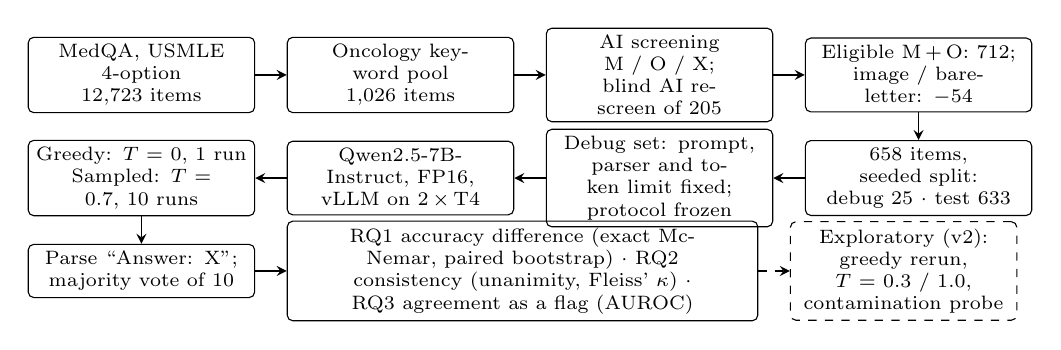
\begin{tikzpicture}[
  node distance=3.5mm and 4mm,
  box/.style={draw, rounded corners=2pt, align=center, font=\scriptsize, inner sep=2.5pt, text width=#1},
  box/.default=27mm,
  arr/.style={->, >=stealth, semithick}]
\node[box] (medqa) {MedQA, USMLE 4-option\\\medqaN{} items};
\node[box, right=of medqa] (pool) {Oncology keyword pool\\\poolN{} items};
\node[box, right=of pool] (screen) {AI screening M / O / X;\\blind AI re-screen of \screenN{}};
\node[box, right=of screen] (elig) {Eligible M\,+\,O: \eligibleN;\\image / bare-letter: $-$\excludedN};
\node[box, below=of elig] (split) {\finalN{} items, seeded split:\\debug \debugN{} $\cdot$ test \nTest};
\node[box, left=of split] (debug) {Debug set: prompt, parser and token limit fixed; protocol frozen};
\node[box, left=of debug] (model) {Qwen2.5-7B-Instruct, FP16,\\vLLM on 2\,$\times$\,T4};
\node[box, left=of model] (arms) {Greedy: $T$ = 0, 1 run\\Sampled: $T$ = 0.7, 10 runs};
\node[box, below=of arms] (parse) {Parse ``Answer: X'';\\majority vote of 10};
\node[box, right=of parse, text width=58mm] (eval) {RQ1 accuracy difference (exact McNemar, paired bootstrap)
  $\cdot$ RQ2 consistency (unanimity, Fleiss' $\kappa$) $\cdot$ RQ3 agreement as a flag (AUROC)};
\node[box, right=of eval, text width=27mm, dashed] (expl) {Exploratory (v2): greedy rerun, $T$ = 0.3 / 1.0, contamination probe};
\draw[arr] (medqa) -- (pool);
\draw[arr] (pool) -- (screen);
\draw[arr] (screen) -- (elig);
\draw[arr] (elig) -- (split);
\draw[arr] (split) -- (debug);
\draw[arr] (debug) -- (model);
\draw[arr] (model) -- (arms);
\draw[arr] (arms) -- (parse);
\draw[arr] (parse) -- (eval);
\draw[arr, dashed] (eval) -- (expl);
\end{tikzpicture}
\Description{A flowchart in three rows. Top row: MedQA items, oncology keyword pool, AI screening with a blind
re-screen, eligible items after exclusions. Middle row, right to left: the seeded split into debug and test sets,
the debug set used to fix and freeze the protocol, the model, and the two decoding arms. Bottom row: answer parsing
and majority vote, evaluation of the three research questions, and the exploratory runs.}
\caption{Study pipeline. Item selection (top row, left to right), protocol freeze and generation (middle row,
right to left), evaluation (bottom row). No model output on test items existed before the protocol was frozen.}
\label{fig:flow}
\end{figure}

\subsection{Items}
Items come from the English, four-option USMLE part of MedQA~\cite{jin2021medqa} on Hugging Face~\cite{medqa_hf}
(\medqaN{} items, pinned commit). A keyword rule (term list in the repository's \texttt{count\_oncology\_items.py}) kept
\poolN{} items with an oncology term in the vignette or the correct answer. Since the pool was drawn from all of MedQA,
the test set mixes items from its train (\nOriginTrain), dev (\nOriginDev) and test (\nOriginTest) splits, which
matters for contamination (Section~\ref{sec:limitations}). An AI screener (Claude Code) coded each item against written
rules: \emph{M}, managing a known or suspected neoplasm or a direct complication; \emph{O}, a neoplasm tested otherwise
(diagnosis, pathology, mechanism, risk, screening, adverse effects of cancer therapy); \emph{X}, incidental. With no
clinical checker available, a second, blind instance of the same model re-coded a random 20\% sample (\screenN{} items)
from the full text; they agreed on \screenAgree{} (Cohen's $\kappa$ = \screenKappa), and the first screener adjudicated
the \adjudicatedN{} disagreements, changing \adjudicatedChanged{} codes (\screenChangedPct\%, our estimate of the
miscoding rate among the \unsampledN{} unsampled items). Of \eligibleN{} eligible items (\codeM{} M, \codeO{} O),
\excludedN{} referring to an image or with bare-letter options were removed; a seeded split left \debugN{} items for
developing the prompt and parser and \nTest{} test items (\nM{} M, \nO{} O). An \emph{objective subset} of \nObjective{}
test items, whose correct answer itself contains an oncology term, depends less on screening judgement.

\subsection{Model, prompt and decoding}
We used Qwen2.5-7B-Instruct~\cite{qwen2024qwen25,qwen25_7b_instruct} at a pinned revision, in 16-bit floating
point, with its own chat template. The system message was \emph{``You are a careful medical expert. Answer the
multiple-choice question.''}; the user message gave the question, the options A--D in the dataset's order, and the
instruction to think briefly, step by step, and end with a line \emph{``Answer: X''}. \emph{Greedy decoding} used
temperature 0 and one output per item; \emph{sampling} drew 10 outputs per item at temperature 0.7, top-$p$ 0.8 and
top-$k$ 20, the model's own defaults. Both used a repetition penalty of 1.05 and at most 512 output tokens; a truncated
output is scored as wrong, which costs the single greedy answer more than the vote, so we also report a lenient
analysis. Seeds were a fixed base plus the item's index; the first 50 test items were run greedily twice.

\subsection{Answer extraction and majority vote}
The answer is the last ``Answer: X'' in the output (Markdown bold allowed), or else the last ``answer is X''; only
a single capital A--D not followed by another letter counts. An output without one is \emph{unparseable} and is
scored as wrong. The \emph{majority vote} is the most frequent letter among the parsed runs; unparseable runs do not
vote, a tie goes to the tied letter that appeared first, and an item with no parsed run has no vote. The \emph{modal
share} is the number of runs giving the voted letter, divided by 10.

\subsection{Outcomes and statistical analysis}
\paragraph{RQ1.} The primary outcome is the accuracy of the majority vote minus that of greedy decoding on the same
items, tested with the exact two-sided McNemar test~\cite{mcnemar1947} on the discordant items ($b$: vote right,
greedy wrong; $c$: the reverse), with a 95\% paired percentile bootstrap CI (10{,}000 resamples). The decision rule
was fixed in advance: \emph{supported} if $p < 0.05$ \emph{and} the lower bound is above 0; \emph{practically
meaningful} if the difference is at least 3 points. A power calculation for the then-planned 684 items gave a minimum
detectable difference of 3.7--4.3 points at a nominal 80\% power (77--78\% in simulation with the exact test) for
12--16\% discordant items. We also report the mean accuracy of a single sampled run and of a majority over the first
$k$ runs ($k$ = 1, 3, 5, 7, 9, 10).
\paragraph{RQ2 and RQ3.} Consistency is described (without a test) by the share of unanimous items, the mean modal
share, Fleiss' $\kappa$~\cite{fleiss1971} over the categories A--D and unparseable, and the pairwise flip rate (the
share of an item's 45 run pairs that disagree), with bootstrap CIs (2{,}000 resamples for $\kappa$ and the AUROC,
10{,}000 otherwise). For RQ3, the AUROC of the modal share for a correct vote is reported; H3 is \emph{supported} if its
lower bound exceeds 0.5, a deliberately modest bar. We also compare accuracy at $\geq$9/10 and $<$9/10 agreement and
plot accuracy against coverage.
\paragraph{Sensitivity.} RQ1 is repeated with unparseable greedy items dropped, on the objective subset, and in the M
and O subgroups (M is descriptive only). Discordant items and items wrong in all 11 generations are analysed. Only
RQ1 is confirmatory; secondary analyses are not corrected for multiple comparisons.

\subsection{Protocol freeze, amendment and post hoc analyses}
The protocol and its decision rules were frozen and committed to the project's repository (commit \texttt{7890add})
before any model output on test items existed, and acceptance criteria for the greedy baseline were written before
the test run. The AI assistant that designed the protocol had read the test items and keys during screening, but no
model output. After validating the baseline, and before looking at the voting comparison, we added an exploratory
amendment as a new protocol version: a greedy rerun of all test items, 10 sampled runs at $T$ = 0.3 and 1.0, and a
contamination probe in which the first wrong option of 100 random test items was hidden and the model asked to
reproduce its exact text (Wilson interval~\cite{wilson1927}). Analyses added after the results were seen, most of them
at the request of a reviewer, are labelled \emph{post hoc}.

% 04_setup -- written by Claude Code (D-045); revised after the peer review (Prompt 16: M1, M6).
\section{Experimental Setup}\label{sec:setup}
Generation ran on Kaggle's free tier with two NVIDIA T4 GPUs (16\,GB each), using vLLM 0.32.0~\cite{kwon2023vllm}
with PyTorch 2.13, tensor parallelism over both GPUs and a context length of 2{,}048 tokens. Both arms were generated
in batches of 64 items, so one engine call held 64 sequences for greedy decoding and 640 for sampling; GPU time
therefore depends on this configuration, and we use output tokens as the measure of cost. Generation took
\genHoursMain{}~h for the main run and \genHoursExtras{}~h for the exploratory run (\sessionHoursMain{} and
\sessionHoursExtras{}~h of GPU session). Each notebook installed pinned versions, cloned the repository at a fixed
commit, checked dataset checksums and ran the unit tests before generating. Evaluation ran on a CPU (Python 3.12,
pandas 3.0, NumPy 1.26, SciPy 1.17), after an audit of the saved outputs (split checksums, no question shared between
debug and test sets, prompts independent of the answer key, identical items, engine, model revision, seeds and token
limit in every arm, chance accuracy with shuffled keys; \auditTotal{} of \auditTotal{} checks passed). Re-running the
evaluation on another machine reproduced the Kaggle result files byte for byte. Greedy decoding on GPUs is not exactly
deterministic (\rerunFiftySame{} of 50 letters were the same in the 50-item rerun) and sampled outputs are not
bit-reproducible. The raw outputs restate licensed question text and are not released; every statistic can be
recomputed exactly from the released parsed answers, and every number in the text is inserted by a script.

% 05_results -- written by Claude Code (D-045); revised after the peer review (Prompt 16: M1, M2, M4, M7, m2, m5-m7,
% m13, m14). Every number is a macro from generated/numbers.tex; tables are generated/tab_*.tex. No item text is quoted.
% Post hoc analyses come from scripts/posthoc_review.py (results/posthoc_review.csv) and are labelled as such.
\section{Results}\label{sec:results}

\paragraph{Output quality.} Every arm answered all \nTest{} test items. \unpGreedyN{} of \runsGreedyN{} greedy
outputs (\unpGreedyPct\%) and \unpSampledN{} of \runsSampledN{} sampled outputs (\unpSampledPct\%) had no
parseable answer; \unpGreedyTruncN{} and \unpSampledTruncN{} of these had reached the 512-token limit, and the
remaining \unpGreedyNotTruncN{} and \unpSampledNotTruncN{}, read during baseline validation, declined to choose an
option. \ties{} votes were decided by the tie rule.

\subsection{RQ1: majority vote versus greedy decoding}
\begin{table}[t]
\caption{RQ1: accuracy (\%) of the majority of 10 sampled runs ($T$ = 0.7) and of greedy decoding on the same
items. $\Delta$ = majority minus greedy in percentage points, 95\% paired bootstrap CI; $b$/$c$ = items right only
with the vote / only with greedy; $p$ = exact McNemar test. Only the first row is confirmatory.}
\label{tab:rq1}
\footnotesize
\begin{tabular}{@{}lrrrrrr@{}}
\toprule
Analysis & $n$ & Greedy \% (95\% CI) & Majority-10 \% (95\% CI) & $\Delta$ points (95\% CI) & $b$/$c$ & $p$ \\
\midrule
All items (confirmatory) & 633 & 67.1 (63.5, 70.8) & 70.6 (67.0, 74.2) & 3.5 (0.9, 6.0) & 46/24 & 0.012 \\
\midrule
Lenient parsing & 625 & 68.0 (64.3, 71.7) & 70.9 (67.2, 74.4) & 2.9 (0.3, 5.4) & 42/24 & 0.036 \\
Objective subset & 271 & 64.9 (59.4, 70.5) & 71.2 (65.7, 76.8) & 6.3 (2.2, 10.7) & 26/9 & 0.006 \\
Management (M) & 118 & 66.9 (58.5, 75.4) & 72.0 (63.6, 79.7) & 5.1 ($-$1.7, 11.9) & 11/5 & 0.21 \\
Other oncology (O) & 515 & 67.2 (63.1, 71.3) & 70.3 (66.4, 74.2) & 3.1 (0.4, 5.8) & 35/19 & 0.040 \\
\bottomrule
\end{tabular}

\end{table}

\begin{table}[t]
\caption{Post hoc analyses of the RQ1 difference: its split into a sampling part and a voting part, the vote against
each single run and against the second greedy run, and the difference by the MedQA split each item came from.}
\label{tab:posthoc}
\footnotesize
\begin{tabular}{@{}lrrrr@{}}
\toprule
Comparison & $n$ & $\Delta$ points (95\% CI) & $b$/$c$ & $p$ \\
\midrule
Single sampled run (mean of 10) $-$ greedy & 633 & 0.9 ($-$1.2, 3.1) & -- & -- \\
Majority of 10 $-$ single sampled run (mean) & 633 & 2.6 (1.1, 4.0) & -- & -- \\
Majority of 10 $-$ each single run (range) & 633 & 1.9 to 3.6 & 39--49/21--35 & 0.007--0.17 \\
Majority of 10 $-$ second greedy run & 633 & 4.1 (1.6, 6.6) & -- & 0.003 \\
\midrule
Majority $-$ greedy, items from the MedQA train split & 492 & 3.5 (0.4, 6.5) & 37/20 & 0.033 \\
Majority $-$ greedy, items from the MedQA dev split & 70 & 2.9 ($-$4.3, 11.4) & 5/3 & 0.73 \\
Majority $-$ greedy, items from the MedQA test split & 71 & 4.2 ($-$1.4, 11.3) & 4/1 & 0.38 \\
\bottomrule
\end{tabular}

\end{table}

The majority vote answered \accVoteMain\% of the test items correctly (95\% CI \accVoteMainLo--\accVoteMainHi)
and greedy decoding \accGreedyMain\% (\accGreedyMainLo--\accGreedyMainHi), a difference of \diffMain{} percentage
points (95\% CI \diffMainLo{} to \diffMainHi; Table~\ref{tab:rq1}); the vote alone was right on \bMain{} items and
greedy alone on \cMain{} (exact McNemar $p$ = \pMain). Under the pre-specified rule, H1 is \emph{supported} and the
point estimate passes the 3-point threshold, but the interval includes smaller gains, and with only \discordancePct\%
discordant items (12--16\% were assumed for power) a significant estimate may overstate the gain. The direction was the
same in every sensitivity analysis: \diffLenient{} points with unparseable greedy items dropped, \diffObjective{} on the
objective subset, \diffO{} in other-oncology items and \diffM{} (\diffMLo{} to \diffMHi) in the \nM{} management items,
the closest proxy for treatment decisions.

The comparison changes decoding and aggregation at once. In a post hoc split (Table~\ref{tab:posthoc}), a single sampled
run was \decompSingle{} points more accurate than greedy decoding (\decompSingleLo{} to \decompSingleHi) and the vote
\decompVote{} points more accurate than a single run (\decompVoteLo{} to \decompVoteHi), so most of the gain is due to
voting; it was similar for items from MedQA's train, dev and test splits, and the vote also beat a second greedy run.
Averaged over 200 random run orders (post hoc), majority-of-$k$ accuracy rose smoothly from \accKOrdOne\% ($k$ = 1) to
\accKOrdThree\% (3), \accKOrdFive\% (5) and \accKOrdTen\% (10), whereas the protocol's first-$k$ curve depends on the run
order (Figure~\ref{fig:k}). The 10 runs used \tokRatio{} times the output tokens of greedy decoding (\tokVoteItem{} vs.\
\tokGreedyItem{} per item).

\begin{figure}[t]
\centering
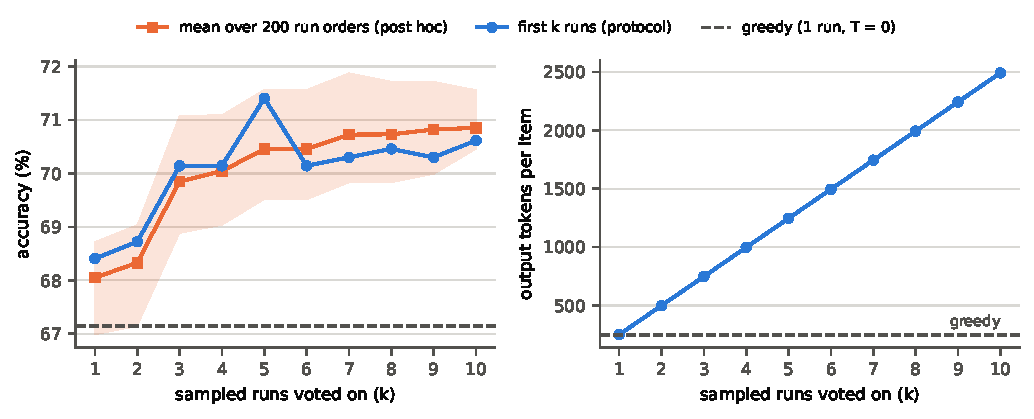
\includegraphics[width=0.86\textwidth]{figures/fig2b_majority_of_k_orders.pdf}
\Description{Two line charts. Left: accuracy of a majority over k sampled runs for k from 1 to 10, as the protocol's
first-k curve and as the mean over 200 random run orders with a shaded band, both above a dashed line for greedy
decoding. Right: output tokens per item growing linearly with k.}
\caption{Majority of $k$ sampled runs. Left: accuracy for the first $k$ runs (protocol) and averaged over 200 random
run orders with the 2.5--97.5 percentile band (post hoc); dashed line: greedy decoding. Right: output tokens per item.}
\label{fig:k}
\end{figure}

\subsection{RQ2 and RQ3: consistency and agreement}
Measured like for like, greedy decoding repeated its letter for \rerunSamePct\% of items, whereas two sampled runs at
$T$ = 0.7 agreed for \pairAgree\%; all ten agreed for only \unanimity\% (Table~\ref{tab:consistency}), with Fleiss'
$\kappa$ \kappaRuns. The distribution of modal shares was broadly similar for management and other items
(Figure~\ref{fig:agree}b).

The modal share separated correct from wrong votes with an AUROC of \auroc{} (95\% CI \aurocLo--\aurocHi), so H3 is
\emph{supported}. When at least 9 of 10 runs agreed (\nGeNine{} items) the vote was correct for \accGeNine\%, otherwise
(\nLtNine{} items) for \accLtNine\%; answering only unanimous items would cover \coverageTen\% of the test set at
\accTen\% accuracy (Figure~\ref{fig:agree}a). The signal needs many runs and partly reflects item difficulty (post hoc,
Table~\ref{tab:consistency}): with only the first 3 runs the AUROC was \aurocFirstThree, whether greedy agreed with the
vote gave \aurocGreedyAgree, and the 10-run modal share predicted the \emph{greedy} answer's correctness about as well
(\aurocGreedyCorrect). \unanimousWrong{} of the \unanimousN{} unanimous items (\unanimousWrongPct\%) were unanimously
wrong.

\paragraph{Shared answer-position preference (post hoc).} Keys were spread evenly over A--D, yet wrong answers rarely
chose A: \wrongAGreedy{} of \wrongGreedyN{} wrong greedy answers (\wrongAGreedyExp{} expected; $p$ = \wrongLettersP) and
\wrongASampled{} of \wrongSampledN{} wrong sampled answers (\wrongASampledExp{} expected). Accuracy was lowest when the key
was A (greedy \accGreedyKeyA\%, vote \accVoteKeyA\%, against \accGreedyKeyOtherMin--\accGreedyKeyOtherMax\% and
\accVoteKeyOtherMin--\accVoteKeyOtherMax\% otherwise). A preference shared by all runs correlates their errors, which
limits what a vote can correct; it may also reflect item content.

\begin{table}[t]
\caption{RQ2 and RQ3 for the 10 sampled runs at $T$ = 0.7 (\nTest{} items); percentile bootstrap CIs over items.}
\label{tab:consistency}
\footnotesize
\begin{tabular}{@{}lr@{}}
\toprule
Measure & Estimate (95\% CI) \\
\midrule
Unanimity, 10/10 runs (\%) & 49.4 (45.5, 53.2) \\
Mean modal share & 0.858 (0.843, 0.872) \\
Fleiss' $\kappa$ across runs & 0.715 (0.689, 0.738) \\
Pairwise flip rate (\%) & 21.4 (19.5, 23.3) \\
AUROC, modal share vs.\ vote correct & 0.737 (0.695, 0.780) \\
Vote accuracy, $\geq$9/10 agree ($n$ = 406) (\%) & 83.5 \\
Vote accuracy, $<$9/10 agree ($n$ = 227) (\%) & 47.6 \\
Coverage / accuracy at 10/10 agreement (\%) & 49.4 / 86.9 \\
\midrule
\multicolumn{2}{@{}l}{\emph{Post hoc comparisons}} \\
Pairwise agreement between two sampled runs (\%) & 78.6 \\
AUROC, modal share of first 3 runs vs.\ vote correct & 0.644 (0.604, 0.685) \\
AUROC, greedy agrees with vote vs.\ vote correct & 0.586 (0.551, 0.621) \\
AUROC, modal share vs.\ greedy correct & 0.749 (0.709, 0.788) \\
\bottomrule
\end{tabular}

\end{table}

\begin{figure}[t]
\centering
\begin{minipage}[b]{0.36\textwidth}\centering
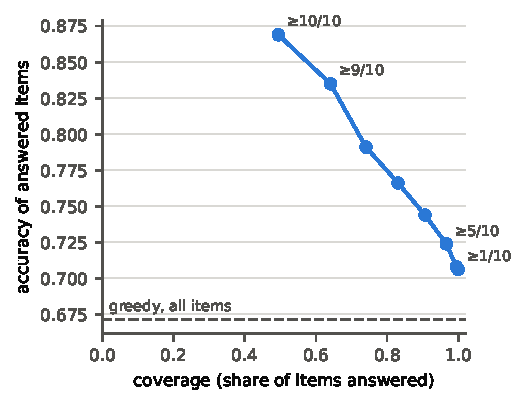
\includegraphics[width=\linewidth]{figures/fig3_accuracy_coverage.pdf}\\(a)
\end{minipage}\hfill
\begin{minipage}[b]{0.45\textwidth}\centering
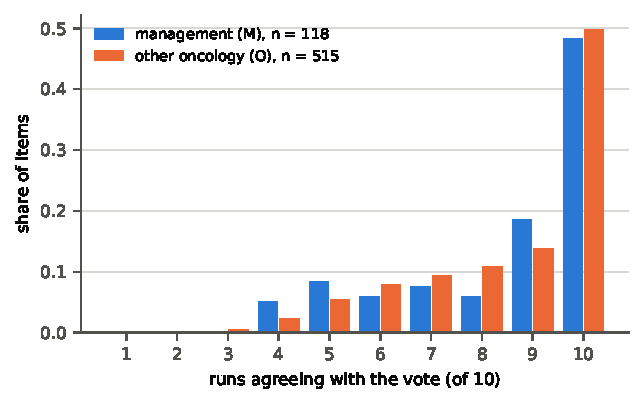
\includegraphics[width=\linewidth]{figures/fig4_modal_share.pdf}\\(b)
\end{minipage}
\Description{(a) A line chart of accuracy against coverage: accuracy rises as fewer items are answered, from the
full test set to items with all 10 runs agreeing, all above a dashed line for greedy decoding. (b) A bar chart of the
share of items by number of runs agreeing with the vote, for management and other items; the largest bars are at 10.}
\caption{(a) Accuracy against coverage when only items with at least $x$ of 10 agreeing runs are answered (dashed:
greedy on all items). (b) Runs agreeing with the vote, for management (M) and other oncology (O) items.}
\label{fig:agree}
\end{figure}

\subsection{Exploratory analyses (protocol amendment)}
A second greedy run of all items scored \accRerun\%, \rerunDiff{} points from the first (\rerunDiffLo{} to
\rerunDiffHi). At $T$ = 0.3 the vote reached \accVoteTLow\% and gained \diffTLow{} points over greedy; its bootstrap
interval (\diffTLowLo{} to \diffTLowHi) excludes zero but the McNemar test does not ($p$ = \pTLow), so it would not
meet the frozen rule, which requires both. At $T$ = 1.0 the vote reached \accVoteTHigh\%, a gain of \diffTHigh{} points
(\diffTHighLo{} to \diffTHighHi; $p$ = \pTHigh). Unanimity was \unanimityTLow\%, \unanimity\% and \unanimityTHigh\% at
$T$ = 0.3, 0.7 and 1.0; in a post hoc paired comparison it was lower at 1.0 than at 0.3 by \unanDiffHighLow{} points
(\unanDiffHighLowLo{} to \unanDiffHighLowHi), while 0.7 and 1.0 did not differ clearly (\unanDiffHighMidLo{} to
\unanDiffHighMidHi). The AUROC stayed between \aurocTLow{} and \aurocTHigh. The contamination probe reproduced the hidden
option exactly for \probeHits{} of \probeN{} items (Wilson interval \probeLo--\probeHi\%), \probeShortHits{} of them
among the \probeShortN{} options of one or two words, which can be guessed.

\subsection{Error analysis}
By construction, on the \bMain{} items where only the vote was right greedy's letter was not the majority letter; the
informative part is how rare it was: it appeared in \bGreedyLetterRunsParsed{} of the 10 sampled runs on average (for
the \bParsedN{} items with a parsed greedy answer), while the correct letter appeared in \bKeyRuns. On the \cMain{}
items where only greedy was right, the correct letter appeared in \cKeyRuns{} of 10 runs. \tiesB{} and \tiesC{} of
these items, respectively, were decided by the tie rule. \allWrong{} items were answered wrongly in all 11
generations: in \allWrongSame{} every generation chose the same wrong option (these are exactly the unanimously wrong
items), \allWrongMixed{} had two or more different wrong options, and \allWrongUnparseable{} mixed a wrong option with
unparseable output.

As an anecdotal check, the AI assistant read two random items per category: greedy sometimes named the right
finding but chose another option; runs sometimes split between two plausible options; in one item several runs
declined to choose; and in always-wrong items every run reasoned towards a non-keyed diagnosis or mechanism. No
clinician checked these readings.

% 06_discussion -- written by Claude Code (D-045); revised after the peer review (Prompt 16: M1, M3, M4, M5, m20).
% Mechanisms are conjectures and are worded as such.
\section{Discussion}\label{sec:discussion}

\paragraph{A modest, uncertain gain, mostly from voting.} The majority of 10 sampled answers was more accurate than a
single greedy answer; the gain is statistically supported and its point estimate passes the threshold set in advance,
but the data are compatible with any gain from \diffMainLo{} to \diffMainHi{} points, it costs \tokRatio{} times the
output tokens, and most of it comes from aggregating runs rather than from sampling itself. Self-consistency was
proposed on the intuition that several reasoning paths converge on the correct answer more often than a single
one~\cite{wang2022selfconsistency}; our data fit this view, since greedy's wrong answers were rare among the sampled
runs, but do not prove a mechanism. A second greedy run, parse failures, ties and the MedQA split of origin do not
change the direction. Strong closed models gained little from voting in
oncology~\cite{holmes2023,stifini2026,windisch2026}; a model that is already consistent has less to gain, which may
explain the difference, but with one model tested this remains a hypothesis.

\paragraph{Consistency depends on the model and its decoding.} Greedy decoding repeated its answer for
\rerunSamePct\% of items, two sampled runs agreed for \pairAgree\%, and unanimity fell between $T$ = 0.3 and 1.0. That
consistency varies with temperature was shown before for small open models~\cite{pinhanez2025} and clinical text
extraction~\cite{liu2026repro}, and that it varies between models in a tumor-board study~\cite{li2025imitation}; we add
the same picture for reasoning outputs on oncology questions. Our figures cannot be ranked against the ChatGPT
tumor-board studies~\cite{liao2025,asoglu2026} (real cases, free text, three runs, unreported settings), and our 9-of-10
stability (\stableTHigh--\stableTLow\%) is only loosely comparable with letter-only answers~\cite{pinhanez2025}. The
number of runs and their consistency, which our review recommended reporting~\cite{sharma2026review}, can only be
interpreted together with the decoding settings.

\paragraph{Agreement is a weak signal.} Agreement tracked correctness (AUROC \auroc), but it needs many runs, partly
reflects item difficulty, and \unanimousWrongPct\% of unanimous answers were wrong, all of them also wrong under greedy
decoding. Such systematic errors, presumably gaps in knowledge or reasoning, and the runs' shared preference against
option A are invisible to both voting and agreement.

\paragraph{Implications.} These results concern exam questions with a single keyed answer, not board decisions, and say
nothing about patient care or clinical use of model output. For studies that compare LLMs with tumor boards they
support one reporting practice: state how many times each case was run, with which decoding settings, and how
consistent the runs were.

% 07_limitations -- written by Claude Code (D-045); revised after the peer review (Prompt 16: M2, M3h, M7, m1, m4, m15).
\section{Limitations}\label{sec:limitations}
\emph{Exam questions are a proxy.} MedQA items have one keyed answer and were written for a licensing exam; a tumor
board weighs imaging, pathology, staging, comorbidity, guidelines and the patient's wishes, often accepts more than one
option, and decides by discussion. Only \nM{} of our \nTest{} items concern management, and their result is imprecise.
Nothing here measures clinical usefulness or safety.

\emph{Contamination.} Most test items (\nOriginTrain{} of \nTest) come from MedQA's training split, which is widely
redistributed; whether the model saw them is unknown. The probe is weak (one hidden option, exact match, no control
set, many short options). Memorised items would raise accuracy and could make runs agree more, which would shrink, not
protect, the voting gain; similar gains in items from MedQA's train, dev and test splits argue against a large effect,
but those strata are small.

\emph{Screening by AI.} Oncology relevance was coded by an AI model and checked on a sample by a second, blind instance of
the same model, whose errors may be correlated with the first; the first screener adjudicated. The objective subset
gave a result in the same direction.

\emph{One model, prompt, option order and seed set.} The runs share a preference against option A, so their errors
are not independent; shuffling the options per run, a second seed set and a second model are the obvious next tests.

\emph{Statistics and literature.} Only RQ1 is confirmatory; other analyses are not corrected for multiple comparisons.
Fewer items were discordant than the power calculation assumed, so the estimate may be inflated, and the management
subgroup cannot detect gains below roughly 9--10 points. The 3-point threshold is our own choice. Several cited studies
were read only as abstracts, and we did not review the literature on benchmark contamination, selective prediction,
answer-position bias or GPU non-determinism.

% 08_conclusion -- written by Claude Code (D-045); revised after the peer review (Prompt 16: M5, §5 items 13-15).
\section{Conclusion}\label{sec:conclusion}
On oncology exam questions, taking the majority of ten sampled answers from a small open model was more accurate than
a single greedy answer, by a modest and uncertain margin (\diffMain{} points, 95\% CI \diffMainLo{} to \diffMainHi)
that comes mostly from voting and costs \tokRatio{} times the output tokens. The model's answers varied from run to run
at its default sampling settings, and their agreement was only a weak signal of correctness, blind to systematic
errors. Studies that compare LLMs with tumor boards should report how often each case was run and with which decoding
settings. Shuffled option orders, other open models and free-text recommendations on real board cases are the natural
next tests.

% 09_statements -- written by Claude Code (D-045); revised after the peer review (Prompt 16: M6, m18).
% The AI-use statement must stay accurate (Prompt 18). Open items (O-8: course policy) are tracked in the decision log.
\section*{AI-Use Disclosure}
This study was carried out with extensive help from an AI assistant, Claude Code (Anthropic; Claude Opus 5.5), as part
of a course on AI tools for research. The assistant proposed candidate gaps and designs, wrote the code, ran the GPU
jobs, screened the items and adjudicated disagreements with a second, blind instance of the same model, analysed the
results and wrote this manuscript; a further instance that had not written it reviewed the draft, and the assistant
revised it after checking each point. The author chose the research gap, design and baseline, approved the frozen
protocol and every amendment, and is responsible for the content; these decisions are logged with dates. No clinician
reviewed the items or outputs. References were built from DOI, PubMed or arXiv records, but several were read only as
abstracts; every number was inserted by a script from the saved results.

\section*{Data and Code Availability}
Code, configuration files (including the protocol frozen at commit \texttt{7890add}), item identifiers, screening
codes, parsed answers and all derived results are available at
\url{https://github.com/vibhum-phd/lab7-oncology-llm-voting}. The MedQA question text is not redistributed, because
the licence of the original data is not stated; it can be downloaded from the pinned dataset commit~\cite{medqa_hf}.
The raw model outputs restate question text and are therefore not released.


\bibliographystyle{ACM-Reference-Format}
\bibliography{refs}

\end{document}
